\documentclass[12pt,a4paper]{article}
\usepackage[utf8]{inputenc}
\usepackage[spanish]{babel}
\usepackage{amsmath}
\usepackage{amsfonts}
\usepackage{amssymb}
\usepackage{makeidx}
\usepackage{hyperref}
\usepackage{graphicx}
\usepackage{fancyhdr}
\usepackage{wrapfig}
\usepackage{caption}
\usepackage{subcaption}
\usepackage{float}
\usepackage{placeins}
\usepackage{listings}
\usepackage{afterpage}
\usepackage[export]{adjustbox}
\usepackage{multicol}
\usepackage[left=2cm,right=2cm,top=2cm,bottom=2cm]{geometry}
\graphicspath{ {./images/} }

\title{Gymodo}

\pagestyle{fancy}
\fancyhf{}
\rhead{Gymodo}
\lhead{M13 Proyecto Desarrollo de aplicaciones multiplataforma}
\fancyfoot[C,CO]{\leftmark}
\fancyfoot[L,RO]{\thepage}

\renewcommand{\headrulewidth}{2pt}
\renewcommand{\footrulewidth}{1pt}

\lstset{
  language=bash,
  basicstyle=\ttfamily
}


\begin{document}

\begin{titlepage}
    \begin{center}
        \vspace*{1cm}
            
        \Huge
        \textbf{Gymodo}
            
        \vspace{0.5cm}
        \LARGE
        La mejor App para tu gym
        
        
\includegraphics[width=\textwidth]{gymodo_logo}
        
        \vfill
        

        Edgar Luque, Shah Sawar, Ronald Intriago\\
            
        \vspace{0.8cm}
           
            
        \Large
        Desarrollo de Aplicaciones Multiplataforma\\
        Escola del Treball\\
        Barcelona\\
        \today
            
    \end{center}
\end{titlepage}

\newpage

\begin{abstract}
Gyomodo es una aplicación que tiene como objetivo resolver los problemas que puedan tener los gymnasios en estos tiempos modernos, pero sobretodo, problemas originados a partir de la pandemia del Covid-19.

Este documento explica el desarrollo de esta aplicación, su funcionalidad y la organización del equipo.
\end{abstract}

\newpage

\tableofcontents

\newpage

\section{Presentación del proyecto}
Este proyecto se basa en el desarrollo de una aplicación para Android, esta aplicación tiene como objetivo principal cubrir las necesidades digitales que puede tener un gimnasio como:

\begin{itemize}
\item Crear rutinas y ejercicios.
\item Reservar una hora para ir al gimnasio.
\item Crear tus propias dietas y escanear el código de barras de los productos para ver su nutrientes.
\item Ver noticias relacionadas con el mundo del ejercicio.
\end{itemize}

La función que creemos mas importante es la de reservar hora en un gimnasio, ya que en estos tiempos de pandemia se puede requerir pedir hora previa antes de ir a un gimnasio.

Usando la librería \textbf{ML Kit} de Google podemos escanear el código de barras que tienen los productos, esto nos da una id que podemos usar para buscar el producto usando la API del servicio \textbf{Open Food Facts} que es una base de datos abierta sin animo de lucro con información sobre productos alimenticios "hecha por todos y para todos".

El código esta disponible en github: \href{https://github.com/Gymodo}{https://github.com/Gymodo}

\newpage

\section{Estructura y Organización}
TODO EXPLICAR ORGANIZACION AQUI

\newpage

\section{Tecnología usada}

\subsection{Organización}

\subsubsection{Asana}


\begin{minipage}{.75\textwidth}
Para organizar las tareas que tenemos que hacer hemos empleado Asana, una aplicación web que permite organizar el trabajo.


Con Asana podemos crear tareas, sub-tareas y asignarlas a cada uno, también permite poner un tiempo limite. 
\end{minipage} %
\begin{minipage}{.25\textwidth}
  
\includegraphics[width=0.7\textwidth, right]{asana}
\end{minipage}


\subsubsection{Toggl}

\begin{minipage}{.75\textwidth}
Para saber el tiempo empleado en cada tarea usamos la herramienta toggl tracker.
\end{minipage} %
\begin{minipage}{.25\textwidth}
  
\includegraphics[width=0.7\textwidth, right]{toggl}
\end{minipage}

\subsection{Desarrollo}

\subsubsection{Control de Versiones}

\begin{minipage}{.75\textwidth}
El sistema de control de versiones que hemos usado es git, gracias a esta herramienta podemos mantener el proyecto de forma eficiente, este es nuestra forma de trabajar:

\begin{enumerate}
\item Actualizar la branca rama principal.
\item Crear una rama donde guardaras tu nuevo trabajo.
\item Hacer el trabajo y subirlo.
\item Otro miembro revisa el código y si está bien se hace un merge a la rama principal.
\item Repetir el paso 1.
\end{enumerate}
\end{minipage} %
\begin{minipage}{.25\textwidth}
  
\includegraphics[width=0.7\textwidth, right]{git}
\end{minipage}


\subsubsection{Android Studio}

\begin{minipage}{.75\textwidth}
Para desarrollar la aplicación hemos usado el IDE Android Studio.
Este IDE es el estándar de la industria para crear aplicaciones de Android, está desarrollada por Google y Jetbrains.
\end{minipage} %
\begin{minipage}{.25\textwidth}
  
\includegraphics[width=0.7\textwidth, right]{androidstudio}
\end{minipage}


\subsubsection{Firebase}

\begin{minipage}{.75\textwidth}
Es una plataforma que te permite crear aplicaciones web y para el móvil, este nos proporciona una base de datos en la nube y una API para interactuar con esta. También nos permite guardar imágenes, ver estadísticas sobre los usuarios que usan la app y más.
\end{minipage} %
\begin{minipage}{.25\textwidth}
  
\includegraphics[width=0.7\textwidth, right]{firebase}
\end{minipage}

\subsubsection{ML Kit}

\begin{minipage}{.75\textwidth}
Es una librería de Google que usa \textit{Machine Learning} y permite realizar acciones como detección de cara, escanear barcodes, identificar objectos, texto, etc.
\end{minipage} %
\begin{minipage}{.25\textwidth}
  
\includegraphics[width=0.7\textwidth, right]{mlkit}
 \end{minipage}

\newpage

\section{Diseño}
El objetivo del diseño es dar al usuario una experiencia fluida y cómoda mientras hace uso de la aplicación, por lo que cada elemento se sitúa en lugares de la pantalla que el usuario encontrará intuitivo.
Además, se han hecho uso del contraste entre colores y varias leyes de Gestalt, tales como la ley de la simetría y la experiencia.

\subsection{Logo}
El logo se compone de un símbolo y texto; el símbolo es un brazo con cierta musculatura levantando una pesa, en este símbolo se puede advertir la forma de un corazón, dando a entender el amor por el \textit{fitness}.
El texto es el nombre de la aplicación usando nuestro color principal y la fuente \textbf{Montserrat} en negrita, el resto de la aplicación también hace uso de ésta.


\subsection{Colores}

Los efectos del ejercicio en el ser humano son positivos; reduce el estrés, la ansiedad y la depresión gracias a la segregación de \textbf{endorfinas}, unas sustancias químicas que producen sensación de felicidad y euforia.

Hemos querido representar esos efectos en nuestro diseño a través del color \textbf{naranja} como color principal, ya que, según la psicología del color, el naranja es energético y se asocia con la juventud, alegría y dinamismo.
Para destacar nuestro color principal y hacer contraste, se han escogido colores oscuros y el blanco. Estos colores oscuros se asocian con la fortaleza; el blanco, con la paz y tranquilidad, estos efectos se consiguen también al tener una vida con una actividad física presente.

\begin{figure}[h]
  \centering
 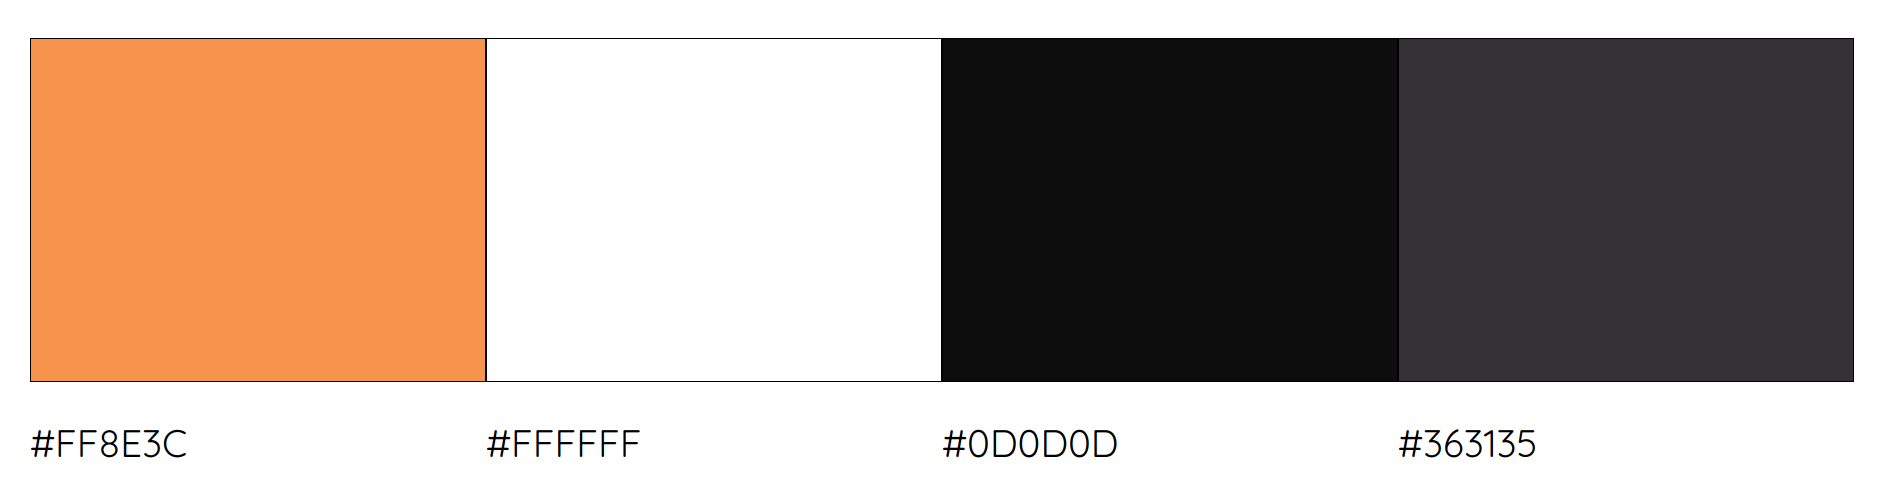
\includegraphics[width=1\textwidth]{color_palette}
 \caption{Paleta de colores}
\end{figure}

\subsection{Mockup}
\href{https://mockittapp.wondershare.com/app/3398ef738f7ac4f35fae5df4eb77004473612d19?simulator_type=device&sticky}{Link al mockup}

todo: poner fotos

\clearpage

\section{Documentación Técnica}

\subsection{Importar el proyecto}

Para importar el proyecto se necesita Android Studio y git.

Primero se clona el repositorio con el código:
\begin{lstlisting}
git clone git@github.com:Gymodo/App.git Gymodo
\end{lstlisting}

Se abre el Android Studio y se importa la carpeta:

\begin{figure}[htb]
    \begin{minipage}[t]{.55\textwidth}
        \centering
        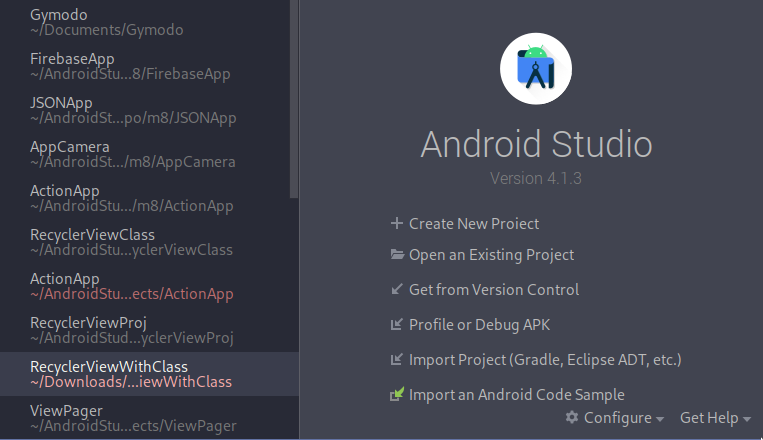
\includegraphics[width=\textwidth]{android-studio-menu1}
        \subcaption{El menu de Android Studio.}\label{fig:androidmenu}
    \end{minipage}
    \hfill
    \begin{minipage}[t]{.35\textwidth}
        \centering
        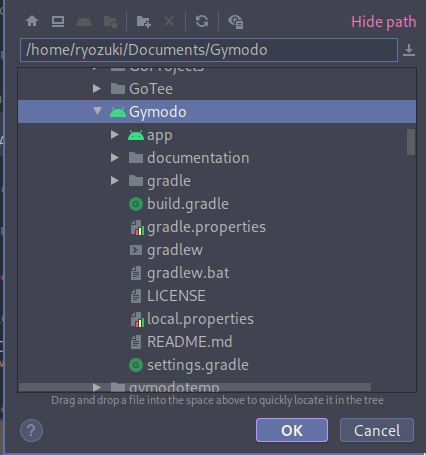
\includegraphics[width=\textwidth]{android-studio-menu2}
        \subcaption{Buscar el proyecto.}\label{fig:androidmenu2}
    \end{minipage}  
    \label{fig:androidimport}
    \caption{Importar el proyecto en Android Studio.}
\end{figure}

Como se ve en la figura \ref{fig:androidmenu} se hace click en \textit{Open an Existing Project} y saldra el menu (figura \ref{fig:androidmenu2}) donde puedes buscar el proyecto.

Una vez cargado el proyecto puedes presionar \textit{shift-f10 }para probar la aplicación.

\subsection{Estructura del código}

El código esta separado en paquetes (que son directorios), estos son los paquetes que tenemos:

\subsubsection{Objectos}
Estos son los objectos que se usan en toda la aplicación

\begin{table}[h!]
\centering
\begin{tabular}{  |l|l| }
\hline
Nombre & Descripción \\
\hline
 Exercise & Representa un ejercicio. \\ 
 \hline
 Muscle & Representa un musculo. \\ 
 \hline
  Serie & Representa una serie de ejercicios. \\ 
 \hline
  Routine & Representa una rutina, que es una serie con información sobre las repeticiones y el peso. \\ 
 \hline
  Diet & Representa una dieta, que esta formada por Meals. \\ 
 \hline
  Meal & Representa una comida del día, formada por varias Foods. \\ 
 \hline
  Food & Representa una comida. \\ 
 \hline
 User & Representa un Usuario. \\ 
 \hline
\end{tabular}
\end{table}


\subsubsection{Adapters}
En este paquete estan las clases que implementan la logica para poder mostrar listas de objectos:

\begin{table}[h!]
\centering
\begin{tabular}{  |l|l| }
\hline
Nombre & Descripción \\
\hline
 CommentsAdapter & Adapter para el object Comments. \\ 
 \hline
 FoodAdapter & Adapter para el objeto Food. \\  
 \hline
 MuscleAdapter & Adapter para el objeto Muscle. \\
 \hline
  NewsAdapter & Adapter para el objeto News. \\
 \hline
  PostsAdapter & Adapter para el objeto Post. \\
 \hline
  ReservationAdapter & Adapter para el objeto Reservation solo con las horas. \\
 \hline
 SeriesAdapter & Adapter para el objeto Serie. \\
 \hline
 SeriesSelectAdapter & Adapter para el objeto Serie con selección. \\
 \hline
 UserReservationsAdapter & Adapter para el objeto Reservation con todo. \\
 \hline
 ViewPagerAdapter & Adapter para los fragment. \\
 \hline
 WorkoutAdapter & Adapter para el objeto Workout. \\
 \hline
\end{tabular}
\end{table}


\clearpage


\subsection{Diagrama UML}

\begin{figure}[h]
 	\centering
	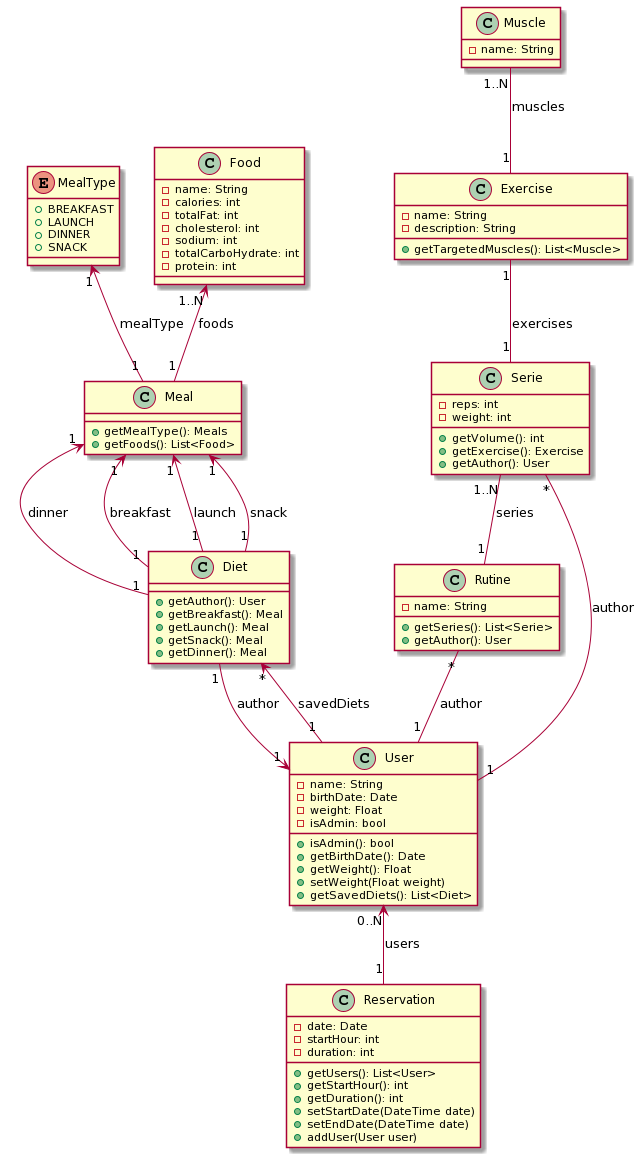
\includegraphics[width=0.6\textwidth]{uml}
	\caption{Diagrama UML}
\end{figure}

\newpage

\subsection{Diagrama Casos de Uso}

\begin{figure}[h]
 	\centering
	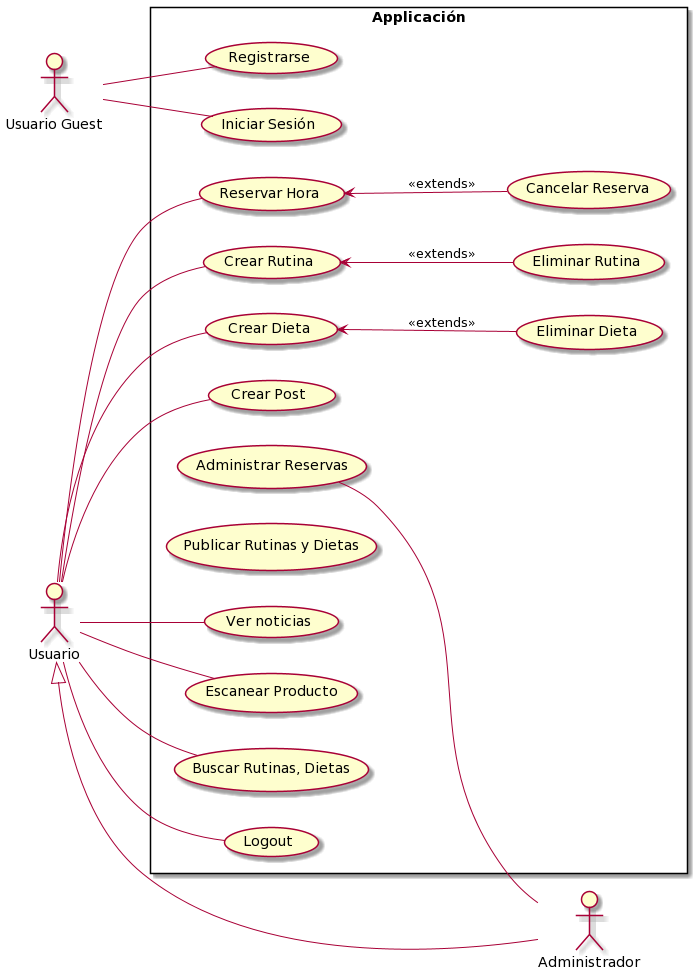
\includegraphics[width=0.8\textwidth]{casos_uso}
	\caption{Diagrama de Casos de Uso}
\end{figure}

TODO: Explicar casos de uso paso a paso. e.g: 1. seleccionar boton x, hacer x, etc

\newpage

\subsection{Diagrama Relacional (bases de datos)}

\begin{figure}[h]
 	\centering
	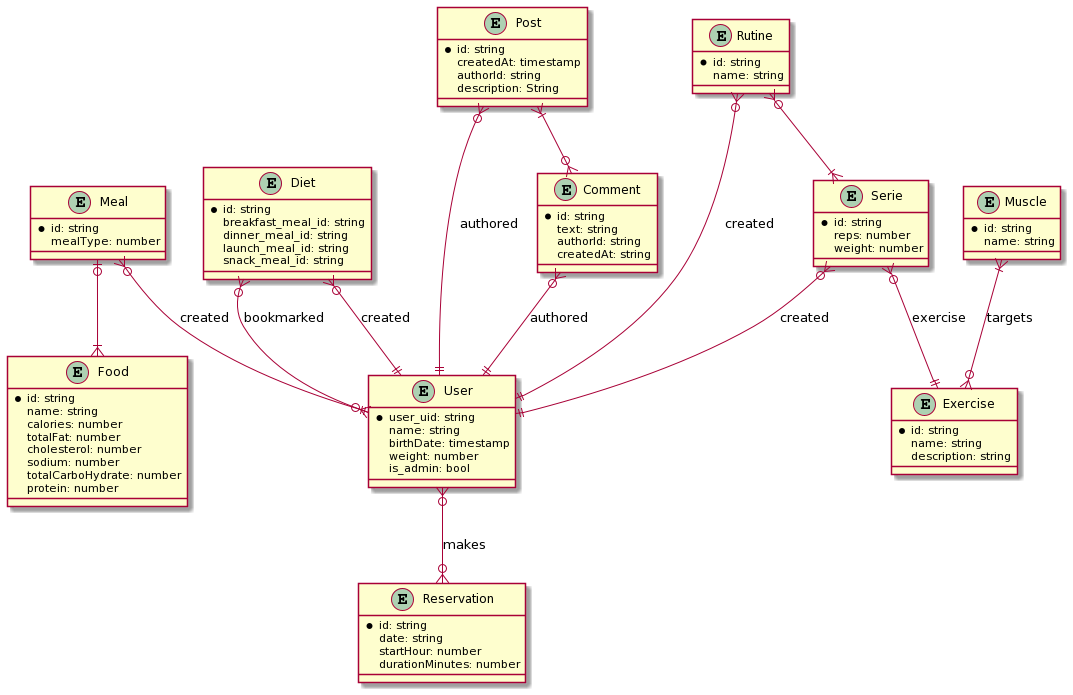
\includegraphics[width=\textwidth]{diagramaer}
	\caption{Diagrama Entidad Relacion}
\end{figure}

\clearpage

\subsection{Manual de usuario}
Explicar como usar la app, alomejor poner alguna foto.

\newpage

\section{Estadísticas sobre el proyecto}

\subsection{Contribuciones}

\begin{figure}[h]
 	\centering
	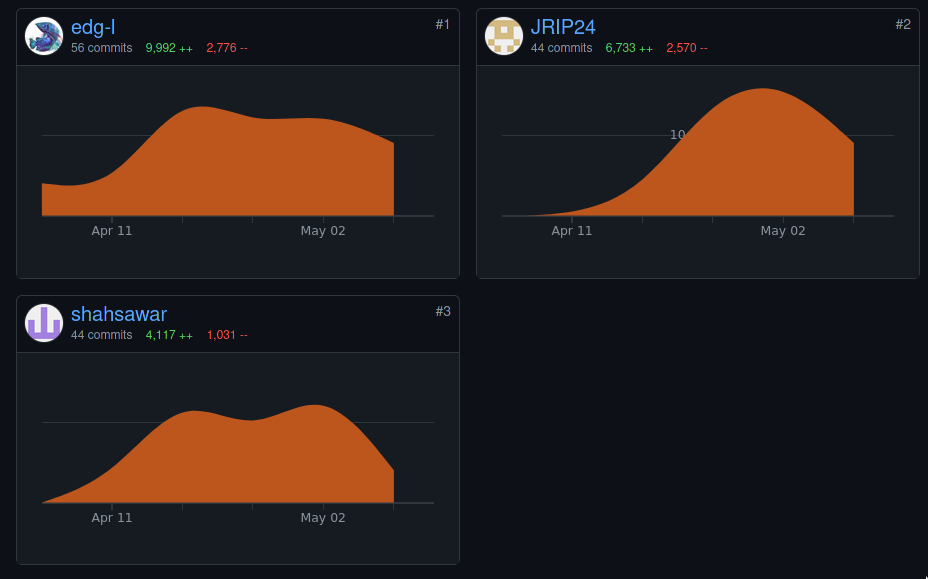
\includegraphics[width=\textwidth]{git-contributors}
	\caption{edg-l = Edgar, JRIP24 = Ronald, shasawar = Shah}
\end{figure}

\subsection{Lineas de código}

\begin{verbatim}
===============================================================================
 Language            Files        Lines         Code     Comments       Blanks
===============================================================================
 Batch                   1           84           61            0           23
 Java                   68         8141         5413         1272         1456
 JSON                    1           47           47            0            0
 Markdown                1            2            0            2            0
 Prolog                  1           21           18            0            3
 Shell                   1          172          130           23           19
 TeX                     1          391          289            0          102
 XML                    97         4248         3747           87          414
===============================================================================
 Total                 171        13106         9705         1384         2017
===============================================================================
\end{verbatim}

\newpage

\section{Conclusión}

\subsection{Posibles ampliaciones}

\subsubsection{Ampliar los datos de la comida}
Se podrían mostrar mas datos sobre la comida que se escanea, y a partir de estos datos llegar a conclusiones útiles para el usuario.

\end{document}